%!TEX root = ../Master_template.tex

\chapter{Introduction}


This chapter addresses the necessity of data augmentation in time series forecasting and classification. It provides a brief overview of augmentation techniques following the formulation of the problem applied in both domains and introduces research problems and questions. The chapter concludes by highlighting the significant contributions of this thesis study.


\section{Data Augmentations}

Synthetic data generation is essential when real original data is limited or insufficient. Data augmentation plays a significant role in creating additional samples by applying various transformations or modifications to the original data. These techniques significantly enhance the original dataset by introducing a wider variety of patterns, which improves the model's generalizability and helps reduce errors and noise.

Time series forecasting is crucial in many areas, such as finance, healthcare, meteorology, and manufacturing.Data augmentation is becoming progressively vital in time series forecasting, as it plays a key role in boosting model accuracy and strengthening generalization capabilities~\cite{chen2023fraugfrequencydomainaugmentation, arabi2024wavemaskmixexploringwaveletbasedaugmentations}. On the other hand, time series classification is important in health care, social security, human activity recognition, remote sensing, and numerous other areas~\cite{Ismail_Fawaz_2020}. Many different augmentation techniques have been studied and designed for both domains. 

Section~\ref{section:formulation} formulates the problem for both time series forecasting and classification settings, whereas Section~\ref{sec: approaches} describes the most essential existing augmentation techniques.






\section{Problem Formulation} \label{section:formulation}

\subsection*{Multivariate Time Series Forecasting}


Multivariate time series prediction forecasts future values for multiple interconnected variables or channels over time. The forecasting problem is generally classified according to the prediction horizon length: long-term forecasting (e.g., 96 or more time steps ahead) and short-term forecasting (e.g., 12 or fewer time steps ahead). The prediction horizon for long-term forecasting significantly exceeds that of short-term forecasting tasks, increasing complexity due to increased uncertainties~\cite{liu2024itransformerinvertedtransformerseffective, zhao2024dominantshufflesimplepowerful}.

Formally, a multivariate time series of length $T$ and channel size $C$ is defined as:

\begin{equation}
\mathbf{X} = (x_1, x_2, \dots, x_T) \in \mathbb{R}^{T \times C},
\end{equation}

where each vector $x_i \in \mathbb{R}^{C}$ represents observations across all channels at the $i$-th timestamp.

Time series data are partitioned into training, validation, and test subsets according to the specific proportions for each dataset.
For simplicity, training data is considered the entire sequence in this formulation. There are many $\mathbf{X} $ sets in the training dataset; for simplicity, we take one set to describe. Furthermore, all possess a batch dimension; however, for the sake of simplicity, it is considered one in our formulation.


Given a look-back window $\mathbf{L}$ containing past observations up to timestamp $t < T$:

\begin{equation}
\mathbf{L} = (x_1, x_2, \dots, x_t) \in \mathbb{R}^{t \times C},
\end{equation}

the objective is to predict the future target horizon $\mathbf{F}$, defined as:

\begin{equation}
\mathbf{F} = (x_{t+1}, x_{t+2}, \dots, x_{T}) \in \mathbb{R}^{(T - t) \times C}.
\end{equation}

A model $f_{\boldsymbol{\theta}}$ parameterized by $\boldsymbol{\theta}$ is learned to approximate the mapping from the look-back window to the forecast horizon:

\begin{equation}
f_{\boldsymbol{\theta}}: \mathbb{R}^{t \times C} \rightarrow \mathbb{R}^{(T - t) \times C}, \quad \mathbf{L} \mapsto f_{\boldsymbol{\theta}}(\mathbf{L}).
\end{equation}

The goal is to minimize forecasting errors, quantified mainly by Mean Squared Error (MSE):

\begin{equation}
\label{eq: mse}
\text{MSE} = \frac{1}{n}\sum_{i=1}^{n}(y_i - \hat{y}_i)^2,
\end{equation}

where $y_i$ are actual values, $\hat{y}_i$ predicted values, and $n = (T - t) \times C$ the total predicted values across all channels. Mean Absolute Error (MAE) is additionally reported:

\begin{equation}
\text{MAE} = \frac{1}{n}\sum_{i=1}^{n}|y_i - \hat{y}_i|.
\end{equation}



Data augmentation techniques improve model generalization by addressing constraints in the size or representativeness of the look-back window $\mathbf{L}$. Synthetic sequences $\mathbf{S}$, generated through augmentation, enhance training data and facilitate better generalization.



\begin{figure}[h!]
    \centering

\includegraphics[width=1.0\textwidth, height=1.0\textheight, keepaspectratio]{./images/framework_train2.drawio.png}
\caption{Overview of the training pipeline for time series forecasting using augmentation. The look-back window and forecast horizon are first concatenated and then passed through the augmentation module. Synthetic sequences are generated and concatenated batch-wise with the original sequences, effectively doubling the batch size. The model output is compared to the target using the MSE loss, and gradients are backpropagated accordingly. Adapted from the paper~\cite{chen2023fraugfrequencydomainaugmentation}.}

    \label{fig:train_fw}
\end{figure}

Figure~\ref{fig:train_fw} illustrates the training pipeline using augmentation techniques, adapted from~\cite{chen2023fraugfrequencydomainaugmentation}. The look-back window and forecast horizon (target) are combined prior to the implementation of the augmentation techniques. Subsequently, $\mathbf{S}_L$ and $\mathbf{S}_F$ are generated, with the generated look-back window concatenated in batches with the original look-back window, while the forecast horizon is similarly concatenated in batches with the original forecast horizon. The loss (Eq.~\ref{eq: mse}) is computed between the output and the target and subsequently backpropagated to the model. Synthetic sequences are combined in batches with original sequences, thereby effectively doubling the batch size. The augmented input data $\mathbf{\overline{X}}$, with the original input batch size set to one, is defined as:


\begin{equation}
\mathbf{\overline{X}} = [ \mathbf{L}, \mathbf{S_L}] \in \mathbb{R}^{2 \times t \times C}.
\end{equation}

Accordingly, the forecasting model now learns:

\begin{equation}
f_{\boldsymbol{\theta}}: \mathbb{R}^{2 \times t \times C} \rightarrow \mathbb{R}^{2 \times (T - t) \times C}, \quad \mathbf{\overline{X}} \mapsto f_{\boldsymbol{\theta}}(\mathbf{\overline{X}}).
\end{equation}

The primary goal of augmentation is to reduce forecasting errors (MSE and MAE) and improve forecasting accuracy and reliability~\cite{Wen_2021}.

\subsection*{Time Series Classification}

Time series classification forecasts discrete class labels for entire sequences based on their sequentially ordered elements. They can be classified as univariate or multivariate, with univariate involving a single channel and multivariate encompassing multiple channels~\cite{Ismail_Fawaz_2020, gao2024dataaugmentationtimeseriesclassification}.


Formally, a time series for classification with length $T$ and $C$ channels is defined as:

\begin{equation}
\mathbf{X} = (x_1, x_2, \dots, x_T) \in \mathbb{R}^{T \times C},
\end{equation}

where each vector $x_i \in \mathbb{R}^{C}$ represents observations across channels at the $i$-th time step. For the univariate setting, $C = 1$.


The dataset consists of $N$ samples ${\mathbf{X}^{(j)}, Y^{(j)}}_{j=1}^{N}$, with $\mathbf{X}^{(j)} \in \mathbb{R}^{T \times C}$ and corresponding labels $Y^{(j)} \in  \mathbb{R}^{K}$, where $K$ is the number of distinct classes~\cite{Ismail_Fawaz_2020}.

A classification model $g_{\boldsymbol{\phi}}$ parameterized by $\boldsymbol{\phi}$ learns a mapping from input series to discrete labels:

\begin{equation}
g_{\boldsymbol{\phi}}: \mathbb{R}^{T \times C} \rightarrow \mathbb{R}^{K}, \quad \mathbf{X} \mapsto g_{\boldsymbol{\phi}}(\mathbf{X}).
\end{equation}

The goal is to minimize the cross-entropy loss, formally defined as:

\begin{equation} \label{eq: cross}
\mathcal{L}(Y, \hat{Y}) = -\frac{1}{N}\sum_{j=1}^{N}\sum_{k=1}^{K}Y_k^{(j)} \log(\hat{Y}_k^{(j)}),
\end{equation}

where $Y_k^{(j)}$ is a one-hot encoded true label and $\hat{Y}_k^{(j)}$ is the predicted probability for class $k$.

The accuracy metric quantifies the model's performance:


\begin{equation} \label{eq:accuracy}
\text{Accuracy} = \frac{1}{N} \sum_{j=1}^{N} \mathbb{I}\left( \arg\max Y^{(j)} = \arg\max \hat{Y}^{(j)} \right),
\end{equation}

where $\mathbb{I}(\cdot)$ denotes the indicator function that returns $1$ if the predicted class matches the true class and $0$ otherwise~\unskip~\cite{Ismail_Fawaz_2020, ilbert2024dataaugmentationmultivariatetime}.


\begin{figure}[h!]
    \centering
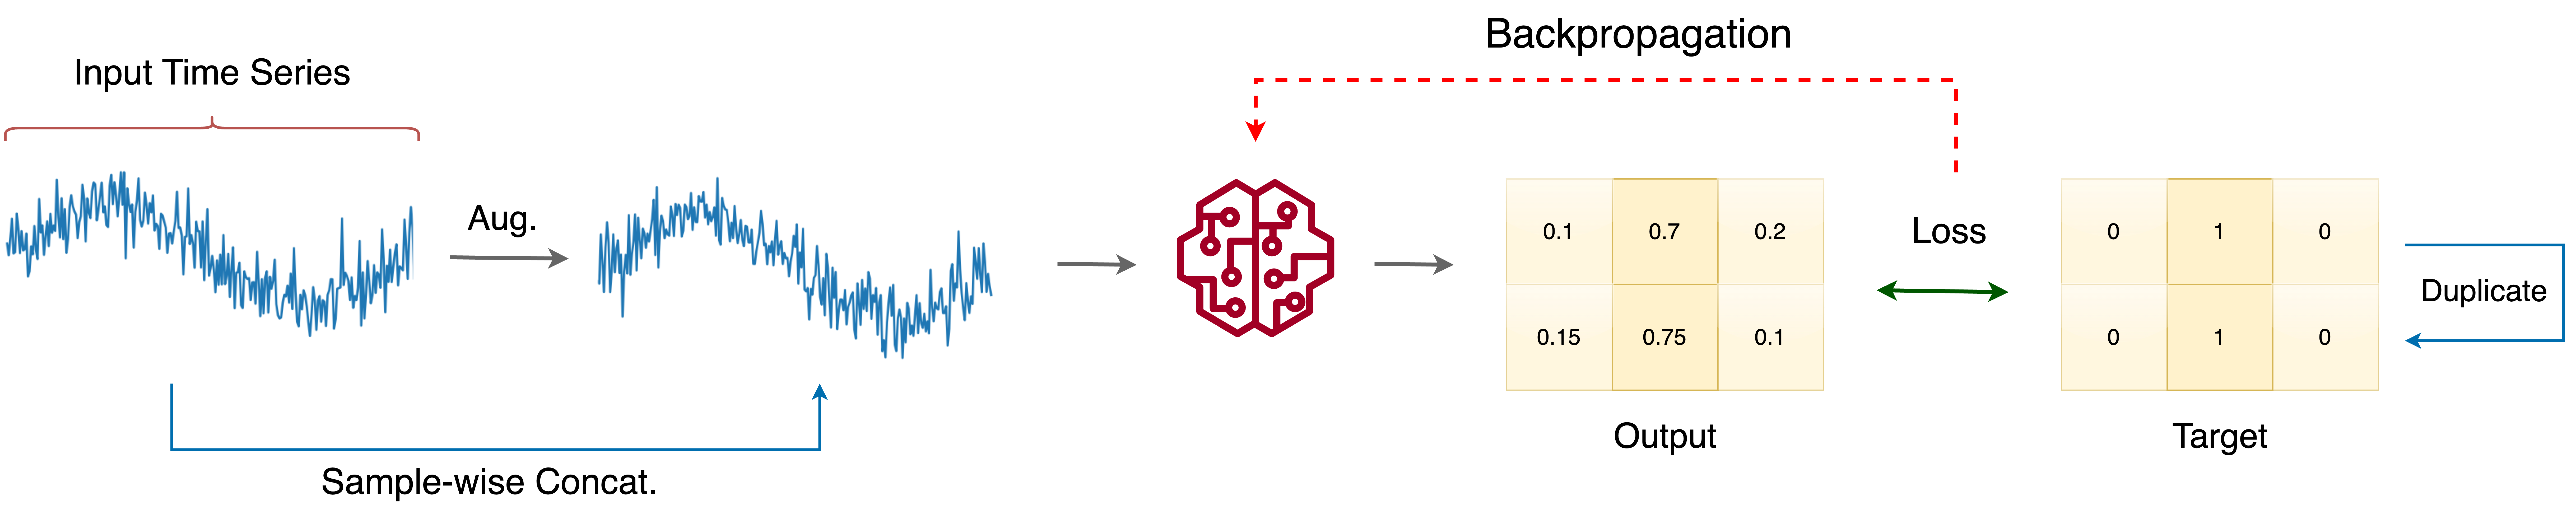
\includegraphics[width=1.0\textwidth, height=1.0\textheight, keepaspectratio]{./images/tsc_framework.drawio.png}

\caption{Training pipeline for time series classification using augmentation. An input sample is passed through an augmentation module to generate synthetic sequences, which are concatenated with the original input on a sample-wise basis—effectively doubling the sample size. Only the inputs are augmented; class labels remain unchanged and are duplicated to match the output. The model computes output probabilities, and the cross-entropy loss is backpropagated. Adapted from the paper~\cite{chen2023fraugfrequencydomainaugmentation}.}

    \label{fig:tsc_fw}
\end{figure}



Figure~\ref{fig:tsc_fw} demonstrates the training pipeline employing augmentation techniques for a single sample, adapted from~\cite{chen2023fraugfrequencydomainaugmentation}. Unlike time series forecasting, only input data $\mathbf{X}$ without class labels undergoes an augmentation process and is concatenated on a sample-wise basis, effectively doubling the sample size. Upon generating the probabilities, the loss (Eq.~\ref{eq: cross}) between the output predictions and the corresponding (duplicated) targets is computed and subsequently backpropagated to the model. Data augmentation techniques for time series classification improve accuracy, minimize loss, and strengthen model robustness and generalization.
 



\section{Approaches} \label{sec: approaches}

% Define all approaches here quickly and define challenges

Numerous augmentation methods have been proposed for time series forecasting, but designing an augmentation technique that maintains temporal dynamics and coherence remains challenging. Augmentation for time series forecasting requires significantly more careful design than augmentation for time series classification~\cite{zhang2023diversecoherentaugmentationtimeseries}. Popular transformation-based augmentations such as jittering, rotation, scaling~\cite{Um_2017}, permutation~\cite{Pan2020}, and window slicing~\cite{leguennec:halshs-01357973} have proven effective for time series classification. However, as described in Section~\ref{section:transformation}, these methods fail to perform well in forecasting tasks due to their disruptive effect on the temporal structure.

Frequency-based augmentations have gained significant popularity for time series forecasting. One of the early approaches, RobustTAD~\cite{gao2021robusttadrobusttimeseries}, applies perturbations to either the magnitude or phase of the frequency spectrum. Methods such as FreqAdd~\cite{freqadd} and FreqPool~\cite{freqpool} were designed following RobustTAD. In FreqAdd, a low-frequency component is selected, and its magnitude is set to half of the maximum magnitude in the corresponding channel, whereas FreqPool compresses the frequency spectrum to focus on dominant frequencies~\cite{freqadd, freqpool}.

Frequency Masking (FreqMask) and Frequency Mixing (FreqMix)~\cite{chen2023fraugfrequencydomainaugmentation} are two of the most widely adopted techniques in recent research. FreqMask involves masking specific components in the frequency domain, while FreqMix combines frequency components based on a defined hyperparameter \textit{rate}~\cite{chen2023fraugfrequencydomainaugmentation}. More recently, Wavelet Masking (WaveMask) and Wavelet Mixing (WaveMix)~\cite{arabi2024wavemaskmixexploringwaveletbasedaugmentations} have been introduced, demonstrating that augmentation can be further improved by using the discrete wavelet transform (DWT) instead of the fast Fourier transform (FFT). Unlike FFT, DWT captures both time and frequency domain characteristics by constructing overlapping time windows~\cite{arabi2024wavemaskmixexploringwaveletbasedaugmentations}. The latest research proposes an augmentation method called Dominant Shuffle~\cite{zhao2024dominantshufflesimplepowerful}, which claims to outperform all previously introduced methods. However, as discussed in Section~\ref{sec: problem}, Dominant Shuffle faces several challenges, including result inconsistency, out-of-distribution issues, and incorrect parameter configurations for model training, which undermine its reported advantages.

In the category of the decomposition-based augmentation methods, Spectral and Time Augmentation (STAug)~\cite{zhang2023diversecoherentaugmentationtimeseries} has shown better performance compared to approaches like weighted Dynamic Time Warping Barycentric Averaging (wDBA)~\cite{asd}, Moving Block Bootstrapping (MBB)~\cite{BERGMEIR2016303}, TimeGAN~\cite{timegan}, and others. STAug uses Empirical Mode Decomposition to decompose the time series and applies weighting in the time domain to generate augmented samples. wDBA and MBB are used for time series classification and forecasting but have failed to demonstrate success compared to frequency and decomposition-based methods for the forecasting tasks~\cite{zhang2023diversecoherentaugmentationtimeseries, chen2023fraugfrequencydomainaugmentation}. Another augmentation method, Upsample~\cite{upsample}, selects consecutive segments from a time series and linearly interpolates them to match the original length. All these augmentation methods for time series forecasting are discussed in detail in Section~\ref{sec: tsf_related}.


In contrast to time series forecasting, transformation-based augmentation methods have achieved success for time series classification tasks. Beyond the previously mentioned augmentation techniques, methods such as magnitude warping, time warping, and window warping have been explored, and window warping is ranked the third most important augmentation method (refer to Table~\ref{tab:augmentation_performance})~\cite{gao2024dataaugmentationtimeseriesclassification}.

Pattern-based augmentation methods, which incorporate transformation techniques to create patterns, have also emerged as some of the most effective strategies for classification tasks. Methods such as SuboPtimAl Warped time-series geNEratoR (SPAWNER)~\cite{s20010098}, wDBA~\cite{asd}, Random Guided Warping (RGW), and Discriminative Guided Warping (DGW)~\cite{iwana2020timeseriesdataaugmentation} rely on Dynamic Time Warping (DTW) or shapeDTW to calculate pair-wise distances. They differ mainly in their strategies for reference selection and use warping techniques to generate augmented samples. Currently, RGW, DGW, and their variants represent the state-of-the-art among augmentation methods for time series classification~\cite{gao2024dataaugmentationtimeseriesclassification}.

Finally, generative model-based and decomposition-based augmentations have been tested for classification tasks but have generally been found ineffective~\cite{gao2024dataaugmentationtimeseriesclassification, 10.1371/journal.pone.0254841}. Consequently, they have been excluded from our experimental protocols. For a detailed analysis of each augmentation method within classification contexts, refer to Section~\ref{sec: tsc_related}.


\section{Research Problem}
\label{sec: problem}

The latest developments in data augmentation for time series forecasting have been characterized by the introduction of innovative techniques, including the most recent Dominant Shuffle. The authors assert that they have overcome the drawbacks of previous augmentation techniques, such as FreqMask/FreqMix, FreqAdd, STAug, and others, commonly facing out-of-distribution challenges. Figure~\ref{fig:ood} depicts this challenge by showcasing t-distributed Stochastic Neighbor Embedding (t-SNE) visualizations of feature spaces derived from various augmentations. The authors assert that Dominant Shuffle diminishes external noise better than other augmentation methods and achieves superior outcomes relative to all current techniques. Additionally, they performed a comprehensive assessment across different model architectures, encompassing both long-term and short-term forecasting tasks, while comparing their augmentation method to the most recent augmentation techniques known to us~\cite{zhao2024dominantshufflesimplepowerful, freqadd, zhang2023diversecoherentaugmentationtimeseries, chen2023fraugfrequencydomainaugmentation}.

\begin{figure}[h!]
    \centering
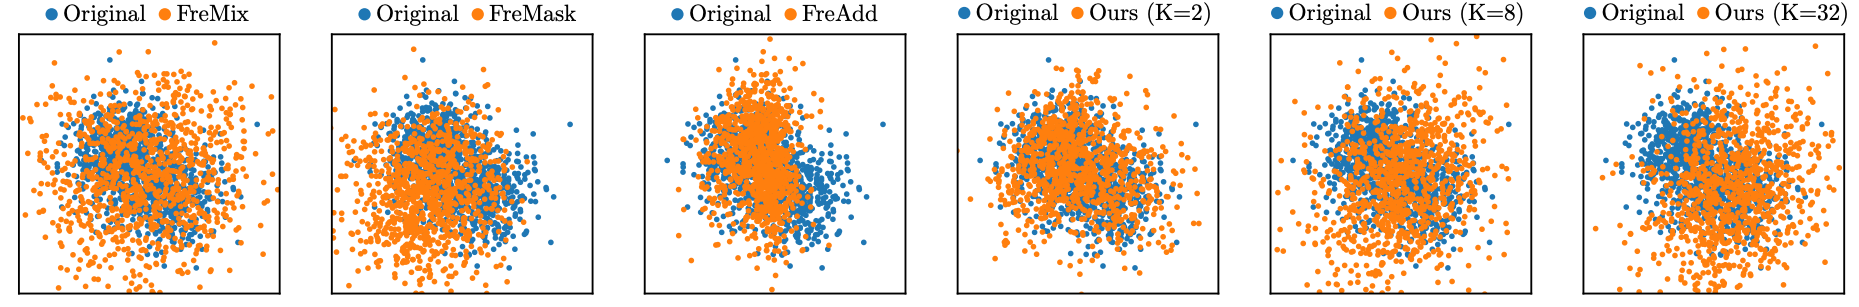
\includegraphics[page=1, width=1.0\textwidth]{./images/ood.png}
    \caption{t-SNE visualization of features of various augmentation methods~\cite{zhao2024dominantshufflesimplepowerful}.}
    \label{fig:ood}
\end{figure}

Despite these claims, several critical issues can be identified in their study. The first major issue is that the authors did not correctly reproduce the original models' hyperparameter settings, as the paper's reviewers reported. This misconfiguration led to a situation where, across many experiments, models trained with augmentations performed worse than their non-augmented counterparts. Additionally, the Dominant Shuffle technique often employed a high shuffling parameter (K), which, as visualized in Figure~\ref{fig:ood}, introduces external noise rather than mitigating it~\cite{zhao2024dominantshufflesimplepowerful}. The second primary concern is the inconsistency of results. When Dominant Shuffle was run multiple times (five different initializations), it frequently failed to achieve the superior performance claimed in the original paper, sometimes even underperforming compared to baseline methods, which is confirmed in our experimentations (see Chapter~\ref{chapter:experiments}). Finally, from a practical standpoint, Dominant Shuffle is computationally expensive relative to other methods like FreqMask/FreqMix and FreqAdd, a finding we confirm in the ablation study (see Table~\ref{tab:augmentation_comparison}) using the publicly available code. Given these observations, there remains a substantial need for a carefully designed augmentation method explicitly tailored for time series forecasting tasks.


The primary aim of this thesis is to design a novel patch-based augmentation method for time series data, drawing inspiration from the successes of similar approaches in the computer vision domain. The goal is not only to achieve superior predictive performance compared to existing time series augmentation methods but also to reduce the external noise introduced by augmentation and to mitigate the domain gap between augmented and original data.  Furthermore, another goal is to establish an augmentation framework applicable across diverse time series tasks, such as time series classification, requiring only minimal modification.

Another important contribution of this thesis is the establishment of a fair experimental protocol, ensuring that the evaluation metrics for models without augmentation match those reported in the original studies. In this way, this thesis provides not only a novel augmentation design but also a rigorous comparative study across both time series forecasting and time series classification domains.


\section{Research Questions}

This master's thesis aims to address the following research questions:

\begin{enumerate}
    \item  How does the proposed patch-based augmentation technique perform compared to existing augmentation methods across various time series forecasting and classification tasks?
    \item  Can the proposed augmentation method enhance model generalization and robustness without introducing significant external noise?
    \item  Can the proposed augmentation framework, with minimal adaptation, be effectively applied to both time series forecasting and classification tasks, providing a flexible solution for future research and applications?
    \item  Are all experimental setups and evaluation protocols implemented fairly to ensure a valid comparison between models with and without augmentation?
\end{enumerate}

These research questions form the foundation for the development, evaluation, and analysis presented throughout this thesis.


\section{Contributions}

The key contributions of this study include:

\begin{itemize}
    \item We propose a novel augmentation method, \textbf{Temporal Patch Shuffle (TPS)}, which consistently outperforms existing augmentation techniques  across seven benchmark datasets for long-term and four for short-term time series forecasting.

    \item TPS not only achieves state-of-the-art results but also improves generalization and robustness while introducing minimal noise, making it a reliable and efficient augmentation strategy.

    \item We extend \textbf{TPS} to the time series classification domain and introduce a new variant, \textbf{Temporal Index Patch Shuffle (TIPS)}, specifically designed for classification tasks. Both TPS and TIPS, individually and in combination, demonstrate superior performance compared to existing augmentation methods on both univariate and multivariate time series classification benchmarks.

    \item We conduct extensive ablation studies to analyze the behavior of our proposed method under various settings, examining their individual components, parameter sensitivity, and robustness to different sources of noise and distribution shifts.

    \item We address flaws in prior experimental protocols by ensuring fair and consistent evaluation, including the correct use of original model hyperparameters within a reasonable computational budget. Additionally, we replicate several augmentation methods from prior works that lacked publicly available code, ensuring reproducibility in the forecasting domain.

    \item Beyond proposing new methods, our master's thesis provides a comprehensive evaluation of existing augmentation techniques, benchmarking them under consistent conditions using recent models for both time series forecasting and classification. 
\end{itemize}
The codebase is available at \url{https://github.com/jafarbakhshaliyev/msc_thesis}.













